\documentclass{standalone}
\usepackage{tikz}

\begin{document}

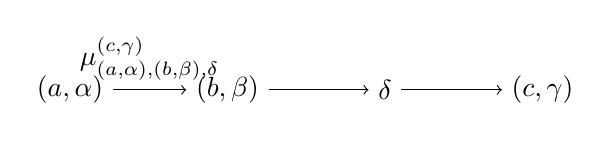
\begin{tikzpicture}[node distance=2cm]

    % Define nodes
    \node (a_alpha) at (0, 0) {$(a, \alpha)$};
    \node (b_beta) at (2, 0) {$(b, \beta)$};
    \node (delta) at (4, 0) {$\delta$};
    \node (c_gamma) at (6, 0) {$(c, \gamma)$};

    % Draw arrows and labels
    \draw[->] (a_alpha) -- node[midway, above] {\(\mu_{(a, \alpha), (b, \beta), \delta}^{(c, \gamma)}\)} (b_beta);
    \draw[->] (b_beta) -- node[midway, above] {} (delta);
    \draw[->] (delta) -- node[midway, above] {} (c_gamma);

\end{tikzpicture}

\end{document}